\documentclass[10pt]{beamer}
\usepackage[utf8]{inputenc}
\usepackage[T1]{fontenc}
\usepackage{amsmath}
\usepackage{amsfonts}
\usepackage{amssymb}
\usepackage{graphicx}
\usetheme{CambridgeUS}

\usepackage{fontspec}
\setmainfont{Arial}
\usepackage{multimedia}
\usepackage{hyperref}

\newcommand{\pptTitle}{Pose Fusion with Chain Pose Graphs for Automated Driving}
\newcommand{\pptShortTitle}{Chain Pose Graphs}
\newcommand{\pptSubTitle}{Reading Report}

\title[(\pptShortTitle)]{\textbf{\pptTitle}}
\subtitle{\pptSubTitle}
\author{HMW-Alexander, Prof. Raj Rajkumar}
\logo{CyLab}
\institute{CMU-ECE}
%\date{}
%\subject{}
\setbeamercovered{transparent}
%\setbeamertemplate{navigation symbols}{}

\begin{document}
	\frame[plain]{\maketitle}
	\begin{frame}{Basic Information}
		\begin{block}{Authors}
			\begin{itemize}
				\item \textbf{Christian Merfels} is with Volkswagen Group Research, Wolfsburg, and Institute of Geodesy and Geoinformation, University of Bonn, Germany.
				\item \textbf{Cyrill Stachniss} is with Institute of Geodesy and Geoinformation, University of Bonn, Germany.
			\end{itemize}
		\end{block}
		\begin{block}{Conference}
			2016 IEEE/RSJ International Conference on Intelligent Robots and Systems (IROS)
		\end{block}
	\end{frame}
	\begin{frame}{Abstract}
		\begin{itemize}
			\item<1-> A \textbf{graph-based} \textbf{multiple localization source fusion} approach.
			\begin{itemize}
				\item A kind of \textbf{Non-Linear Least Squares} optimization method.
				\item Different rates \& Different coverages.
				\item Third-party localization modules.
			\end{itemize}
			\item<2-> \textbf{Sliding window} and \textbf{Chain Pose Graph} guarantee the real-time efficiency.
			\begin{itemize}
				\item Sliding window size controls the number of history nodes be evaluated.
				\begin{itemize}
					\item If size=1, then it becomes a filtering-based solution.
					\item If size=all, then it becomes a batch solution.
				\end{itemize}
				\item Chain Pose Graph avoids the "fill-in" problem while marginalizing nodes.\footnote{At the cost of loosing constraints between non-consecutive nodes.}
				\begin{itemize}
					\item Schur Complement generally fill-in the marginalized system matrix.
					\item Find a marginalization solution with minimal fill-in is NP-complete.
					\item It's helpful for the Cholesky decomposition to solve the final linear solution.
				\end{itemize}
			\end{itemize}
			\item<3-> Experiments
			\begin{itemize}
				\item A real experiment fused the LiDAR, camera, GPS and odometry.
				\item A simulated experiment demonstrated the accuracy's relation to the sliding window size and the number of localization sources.
			\end{itemize}
		\end{itemize}
	\end{frame}

	\begin{frame}{Introduction}
		\begin{block}{Problem \& Solution}
			Individual localization system is not enough (accuracy and coverage), and the combination of orthogonal localization systems is more powerful.
		\end{block}
		\begin{block}{Objective}
			Provides a multi-sensor data fusion approach which is decoupled from the localization algorithm.
		\end{block}
		\begin{block}{Formulation}
			\centering
			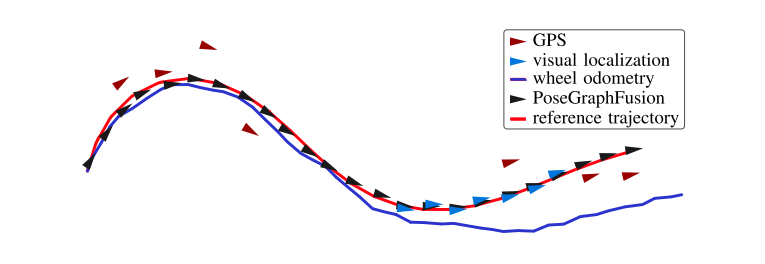
\includegraphics[width=8cm]{./img/posefusion.png}
		\end{block}
	\end{frame}
	
	\begin{frame}{Related Work}
		\begin{block}{Filtering-based appraoches}
			Kalman filter and its variants, particle filter
			\begin{itemize}
				\item Feature: Markov assumption, marginalize all older information.
				\item Problem: Prematurely incorporating the linearization error.
			\end{itemize}
		\end{block}
		\begin{block}{Sliding window smoothing algorithms}
			Compute the ML estimate by Non-Linear Least Squares optimization.
			\begin{itemize}
				\item Feature: consider past measurements
				\item Problem: large window size requires high computation cost.
			\end{itemize}
		\end{block}
	\end{frame}

	\begin{frame}{Method: Pose Graph Fusion}
		\begin{block}{Nonlinear Least Squares Problem}
			$$x^*=\arg\min_x{\sum_{i,j}e_{ij}^T\Omega_{ij}e_{ij}}$$
			\begin{itemize}
				\item $x=[x_1^T,\dots,x_m^T]^T$ is the state vector.
				\item A measurement between $x_i$ and $x_j$:
				\begin{itemize}
					\item $z_{ij}$ is the mean of this measurement
					\item $\Omega_{ij}=\Sigma_{ij}^{-1}$ is the information matrix of this measurement
				\end{itemize}
				\item An error evaluation function $e_{ij}(x_i,x_j,z_{ij})$
			\end{itemize}
			System Matrix and Coefficient Vector
			$$H=\sum_{i,j}{J_{ij}(x)^T\Omega_{ij}J_{ij}(x)},~b^T=\sum_{i,j}e_{ij}^T\Omega_{ij}J_{ij}(x)$$
			Solution:
			$$H\Delta x=-b,~x^*=\hat{x}+\Delta x$$
		\end{block}
	\end{frame}

	\begin{frame}{Method: Pose Graph Fusion}
		\centering
		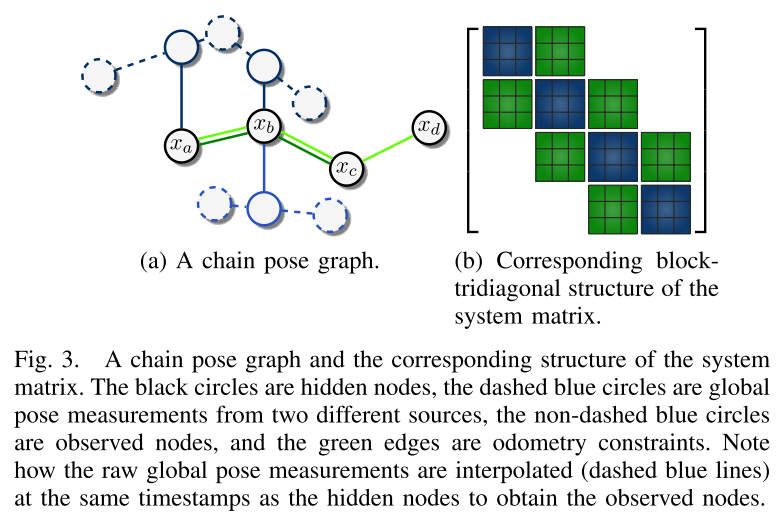
\includegraphics[width=0.7\textwidth]{./img/posegraph.png}
		\begin{itemize}
			\item Measurements are from different localization sources at certain time (interpolation is required)
			\item The odometries information represent the edge between two consecutive state nodes.
		\end{itemize}
	\end{frame}

	\begin{frame}{Method: Time Behavior}
		\centering
		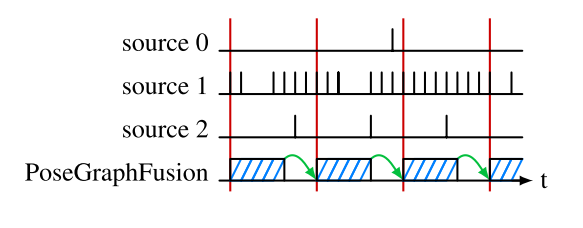
\includegraphics[width=0.7\textwidth]{./img/timebehavior.png}
		\begin{itemize}
			\item The rate of fusion result is constant and is determined by the PoseGraphFusion.
			\item Different window size affects the computation time.
		\end{itemize}
	\end{frame}

	\begin{frame}{Marginalize the Older Nodes}
		\centering
		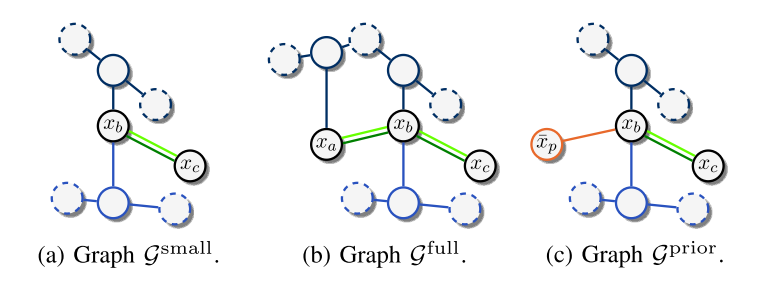
\includegraphics[width=0.7\textwidth]{./img/schur.png}
		\begin{itemize}
			\item (a) directly remove the older node $x_a$, introduce dependency error.
			\item (b) the original full graph.
			\item (c) replace $x_a$ with a virtual prior measurement $\bar{x}_p$.
		\end{itemize}
	\end{frame}

	\begin{frame}{Math about the Marginalization (from full to marginalized)}
		\centering
		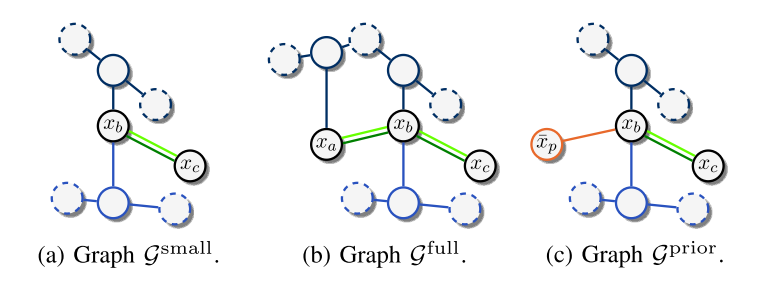
\includegraphics[width=0.5\textwidth]{./img/schur.png}
		\begin{equation}
		H^{small} \Delta x^{small} =\left[\begin{array}{cc}
		H_{bb}^{small} & H_{bc}^{small} \\
		H_{cb}^{small} & H_{cc}^{small} \\
		\end{array}\right] \Delta x^{small} = - \left[\begin{array}{c}
		b_{b}^{small} \\
		b_{c}^{small} \\
		\end{array}\right]
		\end{equation}
		\begin{equation}
		\begin{array}{rcl}
		H^{full} \Delta x^{full} & = & \left[\begin{array}{ccc}
		\bar{H}_{aa} + \hat{H}_{aa} & \hat{H}_{ab} & 0 \\
		\hat{H}_{ba} & H_{bb}^{small} + \hat{H}_{bb} & H_{bc}^{small} \\
		0 & H_{cb}^{small} & H_{cc}^{small} \\
		\end{array}\right] \Delta x^{full} \\
		
		& = & \left(\left[\begin{array}{ccc}
		0 & 0 & 0 \\
		0 & H_{bb}^{small} & H_{bc}^{small} \\
		0 & H_{cb}^{small} & H_{cc}^{small} \\
		\end{array}\right]+\left[\begin{array}{ccc}
		\bar{H}_{aa} + \hat{H}_{aa} & \hat{H}_{ab} & 0 \\
		\hat{H}_{ba} & \hat{H}_{bb} & 0 \\
		0 & 0 & 0 \\
		\end{array}\right]\right) \Delta x^{full} \\
		
		& = & -\left[\begin{array}{c}
		0 \\
		b_b^{small} \\
		b_c^{small} \\
		\end{array}\right] - \left[\begin{array}{c}
		\bar{b}_a+\hat{b}_a \\
		\hat{b}_b \\
		0 \\
		\end{array}\right] = -\left[\begin{array}{c}
		\bar{b}_a + \hat{b}_a \\
		b_b^{small} + \hat{b}_b \\
		b_c^{small} \\
		\end{array}\right]\\ 
		\end{array}
		\end{equation}
	\end{frame}

	\begin{frame}{Math about the Marginalization (Schur Complement)}
		\centering
		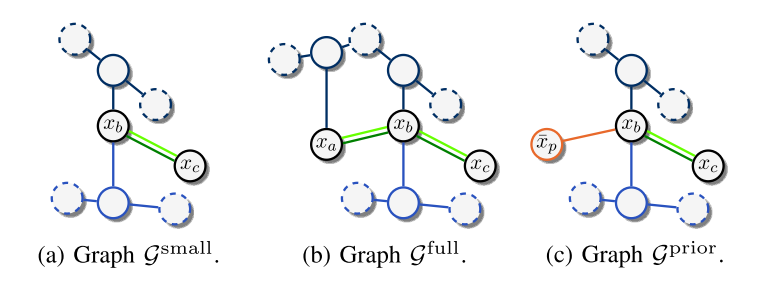
\includegraphics[width=0.5\textwidth]{./img/schur.png}\\
		\begin{equation}
		\begin{array}{rcl}
		\left[\begin{array}{cc}
		\bar{H}_{aa} + \hat{H}_{aa} & \hat{H}_{ab} \\
		\hat{H}_{ba} & \hat{H}_{bb} \\
		\end{array}\right] & \Rightarrow & H^{schur}=\hat{H}_{bb}-\hat{H}_{ba}(\bar{H}_{aa}+\hat{H}_{aa})^{-1}\hat{H}_{ab} \\
		b^{schur}=H^{schur}\Delta x_b & = & \hat{b}_b - \hat{H}_{ba}(\bar{H}_{aa}+\hat{H}_{aa})^{-1}(\bar{b}_a+\hat{b}_a) \\
		\end{array}
		\end{equation}
		\begin{equation}
		\begin{array}{rcl}
		H^{marg} & = & \left[\begin{array}{cc}
		H_{bb}^{small} + H^{schur} & H_{bc}^{small} \\
		H_{cb}^{small} & H_{cc}^{small} \\
		\end{array}\right] \\
		b^{marg} & = & \left[\begin{array}{c}
		b_b^{small} + b^{schur} \\
		b_c^{small} \\
		\end{array}\right]
		\end{array}
		\end{equation}
		\begin{block}{}
			\small
			After the marginalization, the structure of the system matrix is still block-tridiagonal due to the particular design of the chain pose graph, meaning that the sparsity pattern of $H$ is retained after marginalization without fill-in.
		\end{block}		
	\end{frame}

	\begin{frame}{Math about the Virtual Prior Measurement}
		\begin{equation}
		\begin{array}{rcl}
		H^{prior} & = & \left[\begin{array}{cc}
		H_{bb}^{small} + \bar{H}^{prior} & H_{bc}^{small} \\
		H_{cb}^{small} & H_{cc}^{small} \\
		\end{array}\right] \\
		b^{prior} & = & \left[\begin{array}{c}
		b_b^{small} + \bar{b}^{prior} \\
		b_c^{small} \\
		\end{array}\right]
		\end{array}
		\end{equation}
		\begin{equation}
		\begin{array}{rcl}
		e_{pb} & = & \left[\begin{array}{cc}
		R & 0 \\
		0 & 1 \\
		\end{array}\right] (x_b-\bar{x}_p) \\
		J_{pb}(x) & = & \left[\begin{array}{cc}
		R & 0 \\
		0 & 1 \\
		\end{array}\right]
		\end{array}
		\end{equation}
		\begin{equation}
		\begin{array}{rcl}
		\bar{H}_p & = & J_{pb}(x)^T \bar{\Omega}_p J_{pb}(x) = H^{schur}\\
		\Rightarrow \bar{\Omega}_p & = & (J_{pb}(x)^T)^{-1} H^{schur} (J_{pb}(x))^{-1} \\
		\bar{b}_p & = & J_{pb}(x)^T \bar{\Omega}_p e_{pb} = J_{pb}(x)^T \bar{\Omega}_p J_{pb}(x) (x_b-\bar{x}_p) = \bar{H}_p(x_b-\bar{x}_p) \\
		\Rightarrow \bar{x}_p & = & x_b-(H^{schur})^-1 b^{schur} \\
		\end{array}
		\end{equation}
	\end{frame}

	\begin{frame}{Method Summary}
		\begin{itemize}
			\item<1-> Localization sources can be fused in the form of a graph, as well as an adjacent matrix (the system matrix $H$)
			\begin{itemize}
				\item Fusion is decoupled with localization.
				\item Localization is done by non-linear least squares on $H$ and $b$ after fusion. 
			\end{itemize}
			\item<2-> The special design on the Chain Pose Graph makes it easier to be solved.
			\begin{itemize}
				\item Different localization sources are measured at certain timestamps via interpolation
				\begin{itemize}
					\item decouple the measurement relationship between state nodes
					\item handle different rate and coverage problem.
				\end{itemize}
				\item Odometries only connect two consecutive nodes.
			\end{itemize}
			\item<3-> Marginalization enables constant sliding window size, as well as constant final localization rate.
			\begin{itemize}
				\item The Chain Pose Graph's property avoids the fill-in problem during the marginalization.
				\item Compact the marginalized nodes into a virtual prior measurement.
			\end{itemize}
		\end{itemize}
	\end{frame}

	\begin{frame}{Experiment: Real Data}
		\begin{block}{Settings}
			\begin{itemize}
				\item global sources:
				\begin{itemize}
					\item source 0: coarse LiDAR scans to a globally referenced point cloud. (3rd-party)
					\item source 1: GPS (3rd-party)
					\item source 2: visual localization system with a globally referenced feature map.
				\end{itemize}
				\item local source: wheel odometry.
				\item sliding window size: $M=1000$
				\item temporal resolution: $\Delta t=25ms$
				\item experiment route: $16km$ in rural and urban areas in Germany.
			\end{itemize}
		\end{block}
	\end{frame}

	\begin{frame}{Estimation (Baseline: batch solution)}
		\begin{columns}
			\begin{column}{0.5\textwidth}
				Accuracy:
				\begin{itemize}
					\item source 0 (LiDAR): $RMS=1.06m$
					\item source 1 (GPS): $RMS=1.23m$
					\item source 2 (Camera): $RMS=0.28m$
					\item PoseGraphFusion: $RMS=0.38m$
				\end{itemize}
			\end{column}
			\begin{column}{0.5\textwidth}
				Coverage rate:
				\begin{itemize}
					\item source 0: $66.98\%$
					\item source 1 with odometry: $100\%$
					\item source 2: $97.76\%$
					\item PoseGraphFusion: $100\%$
				\end{itemize}
			\end{column}
		\end{columns}		
		\begin{figure}[!ht]
			\centering
			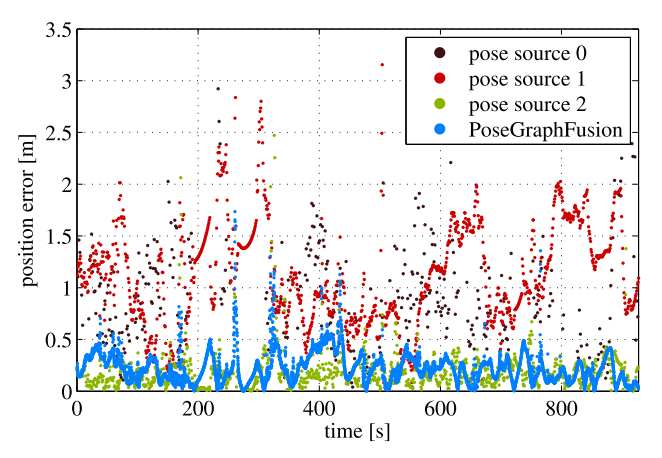
\includegraphics[width=6cm]{./img/error.png}
		\end{figure}
	\end{frame}

	\begin{frame}{Runtime Performance}
		a single core of a laptop with an Intel i7-4800QM processor
		\begin{figure}[!ht]
			\centering
			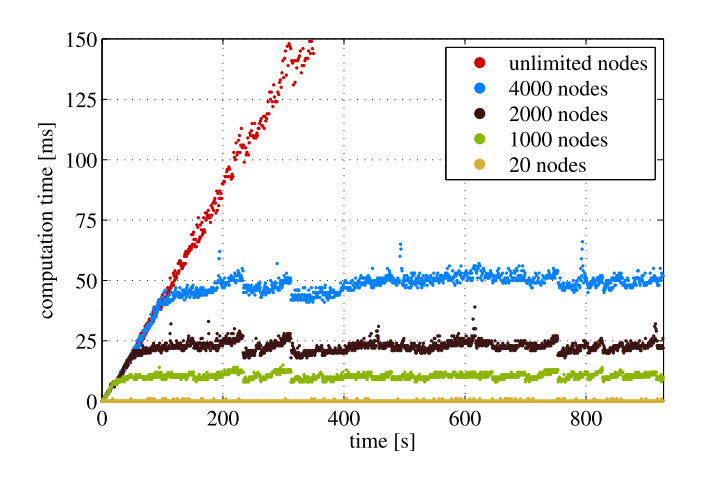
\includegraphics[width=6cm]{./img/runtime.png}\\
			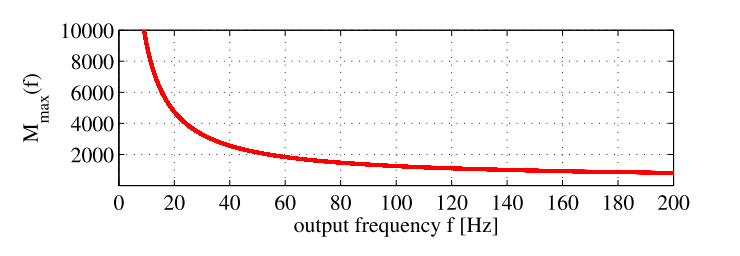
\includegraphics[width=6cm]{./img/relationship.png}
		\end{figure}
	\end{frame}

	\begin{frame}{Sim Data: Number of Hidden Nodes v.s. Accuracy}
		Larger sliding window size $\Rightarrow$ more accurate result
		\begin{figure}[!ht]
			\centering
			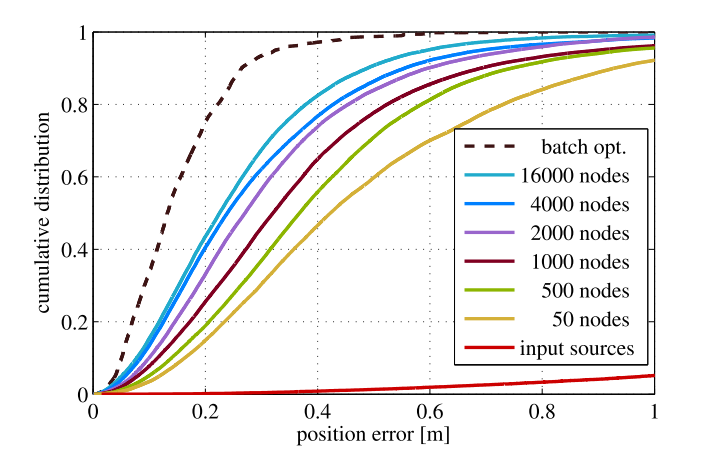
\includegraphics[width=10cm]{./img/accuracy.png}
		\end{figure}
	\end{frame}

	\begin{frame}{Sim Data: Number of Pose Sources v.s. Accuracy}
		More pose sources $\Rightarrow$ more accurate result
		\begin{figure}[!ht]
			\centering
			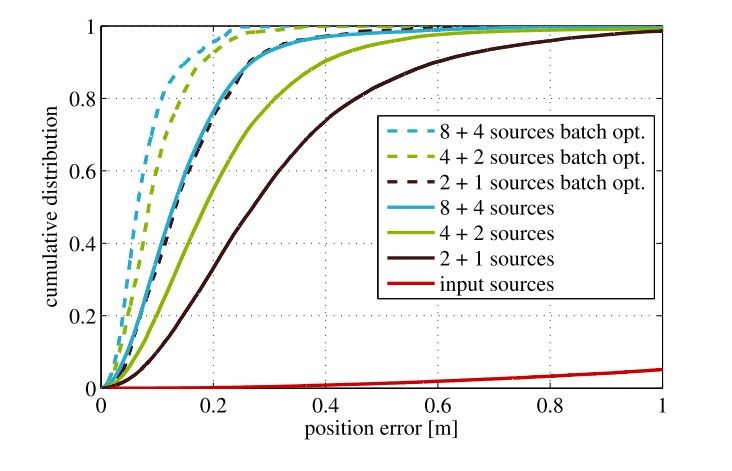
\includegraphics[width=10cm]{./img/sources.png}
		\end{figure}
	\end{frame}

	\begin{frame}{Conclusion Related with CORAL}
		\begin{itemize}
			\item<1-> A graph-based method to fuse different localization sources:
			\begin{itemize}
				\item Multiple GNSS w/ or w/o RTK (global)
				\item Visual place recognition based on landmarks and digital map (global)
				\item Visual odometry (local)
				\item Encoder/IMU (local)
			\end{itemize}
			\item<2-> The paper doesn't prove if all pose sources' coverage rates are low (one is 100\%). We can test it.
			\item<3-> Localization frequency is controllable:
			\begin{itemize}
				\item Relative localization: requires high-frequency and local high-accuracy. Global accuracy is not required. (small sliding window size \& more relative localization modules)
				\item Absolute localization: requires low-frequency and global high-accuracy. Local accuracy is not required. (large sliding window size)
			\end{itemize}
			\item<4-> The possible to COordinate Relative and Absolute Localization:
			\begin{itemize}
				\item The Relative localization graph is a subgraph of the Absolute localization graph.
				\item The bi-directional relationship can be built via the graph.
			\end{itemize}
		\end{itemize}
	\end{frame}
\end{document}